
\section{Codebeispiele}
\subsection{Risikokarte}
\begin{figure}[H]
  \centering
  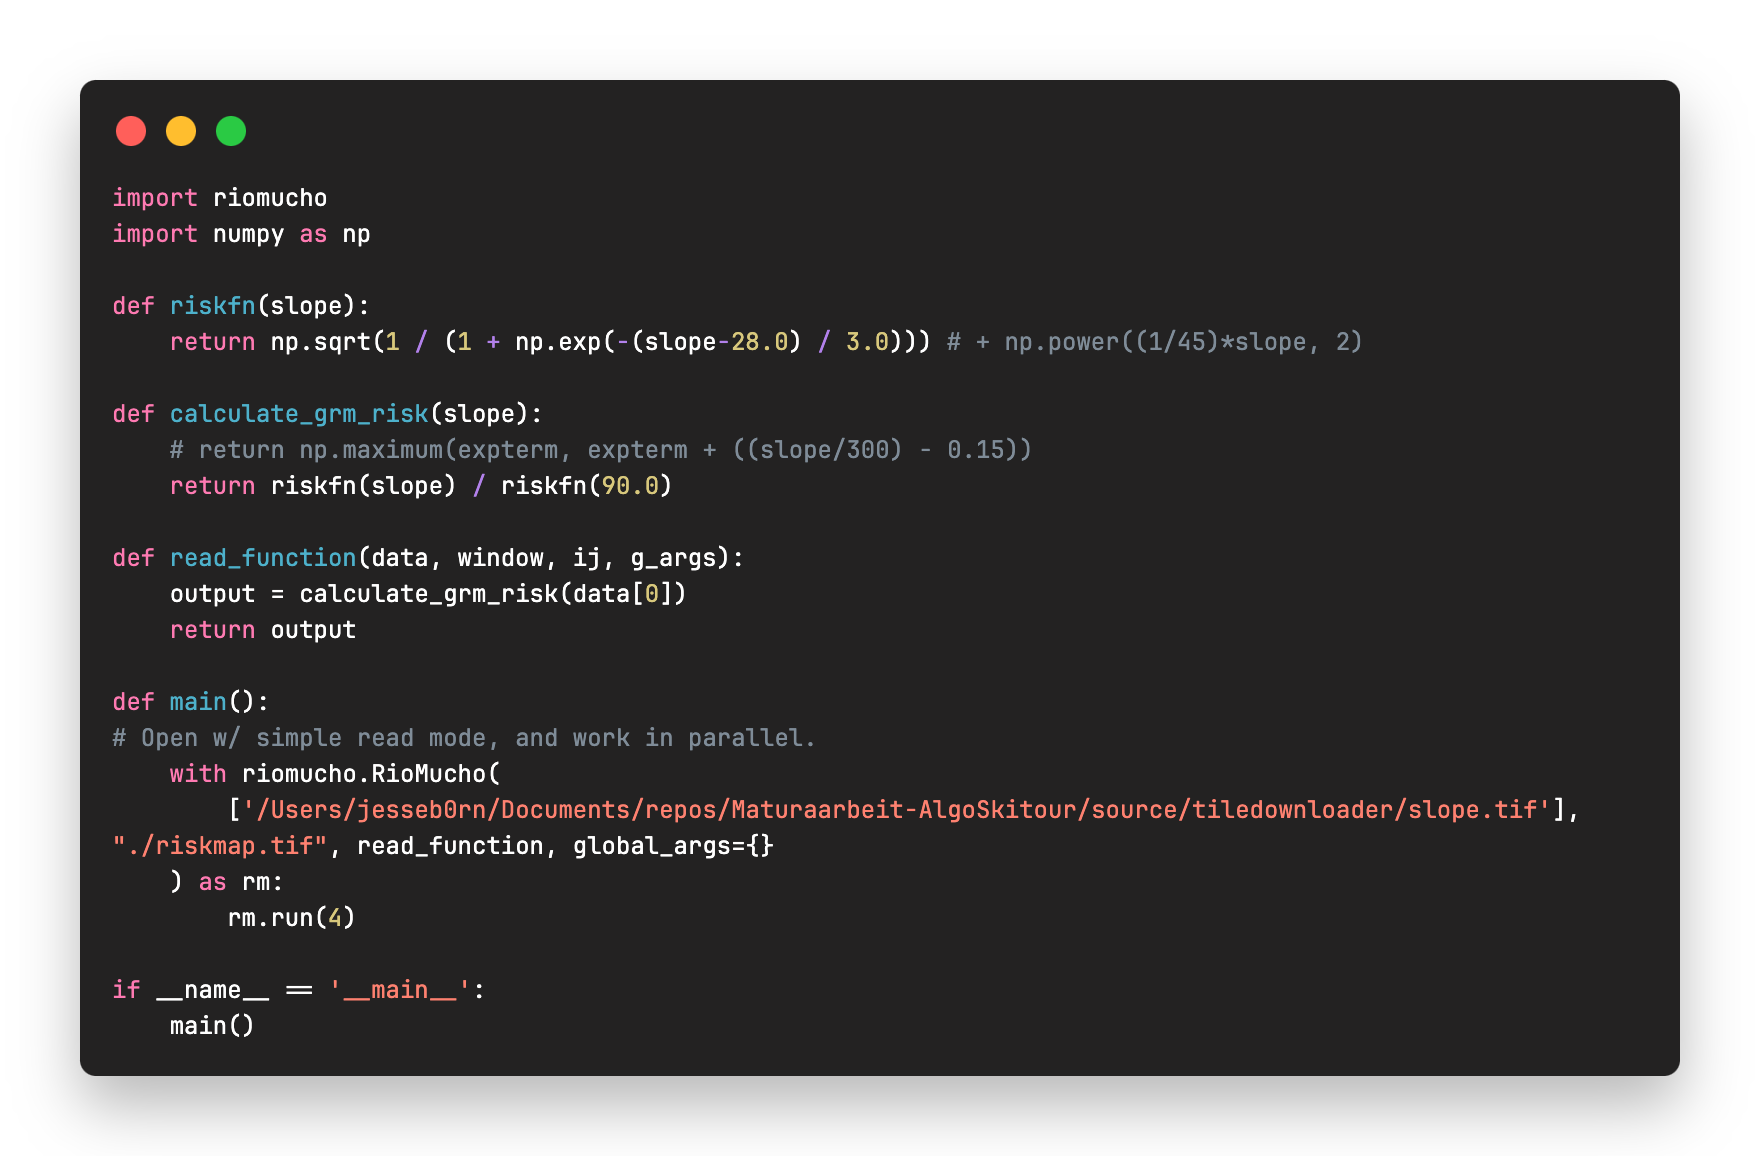
\includegraphics[width=0.9\linewidth]{code}
  \caption{Python Code zur Produktion von Risikokarten aus Neigungskarte}\label{fig:python}
\end{figure}
\section{Formeln zur Berechnung von Oberflächenfaktoren}
Hangneigung und Exposition nach~\cite{gisslopeaspect}:

\begin{equation} \label{eq1}
  \frac{\Delta z}{\Delta x} = \frac{(c + 2f + i) - (a + 2d + g)}{8r}
\end{equation}
\begin{equation} \label{eq2}
  \frac{\Delta z}{\Delta y} = \frac{(g + 2h + i) - (a + 2b + c)}{8r}
\end{equation}

Hangneigung $\rho$ und Exposition $\theta$:
\begin{align}
  \rho &= \arctan \left( \sqrt{
    {\left( \frac{\Delta z}{\Delta x}\right)}^2 + 
    {\left(\frac{\Delta z}{\Delta y}\right)}^2}
  \right)\\
  \theta &= \arctan\left(\frac{\frac{\Delta z}{\Delta x}}{-\frac{\Delta z}{\Delta y}}\right)
\end{align}

Geländekrümmung nach~\cite{gismath}:
\begin{align}
  D &= \frac{{(d + f) / 2 - e}}{{r^2}} \\
  E &= \frac{{(b + h) / 2 - e}}{{r^2}} \\
  F &= \frac{{-a + c + g - i}}{{4r^2}} \\
  G &= \frac{{-d + f}}{{2r}} \\
  H &= \frac{{b - h}}{{2r}}
\end{align}

(6)~--~(10) sind die Faktoren eines teilweisen Polynom vierten Grades~\cite{gismath}.
Hangkrümmung $c_{Plan}$ und $c_{Profil}$ beschreiben, mit welchem Radius sich die Hangneigung parallel (Plankrümmung) bzw.\ senkrecht (Profilkrümmung) zur Exposition ändert:

\begin{align}
    c_{Plan} &= -\frac{{2(DH^2 + EG^2 - FGH)}}{{G^2 + H^2}}
    \\
    c_{Profil} &= \frac{{2(DG^2 + EH^2 + FGH)}}{{G^2 + H^2}}
\end{align}

\section{Evaluationsrouten}\label{app:evalroutes}

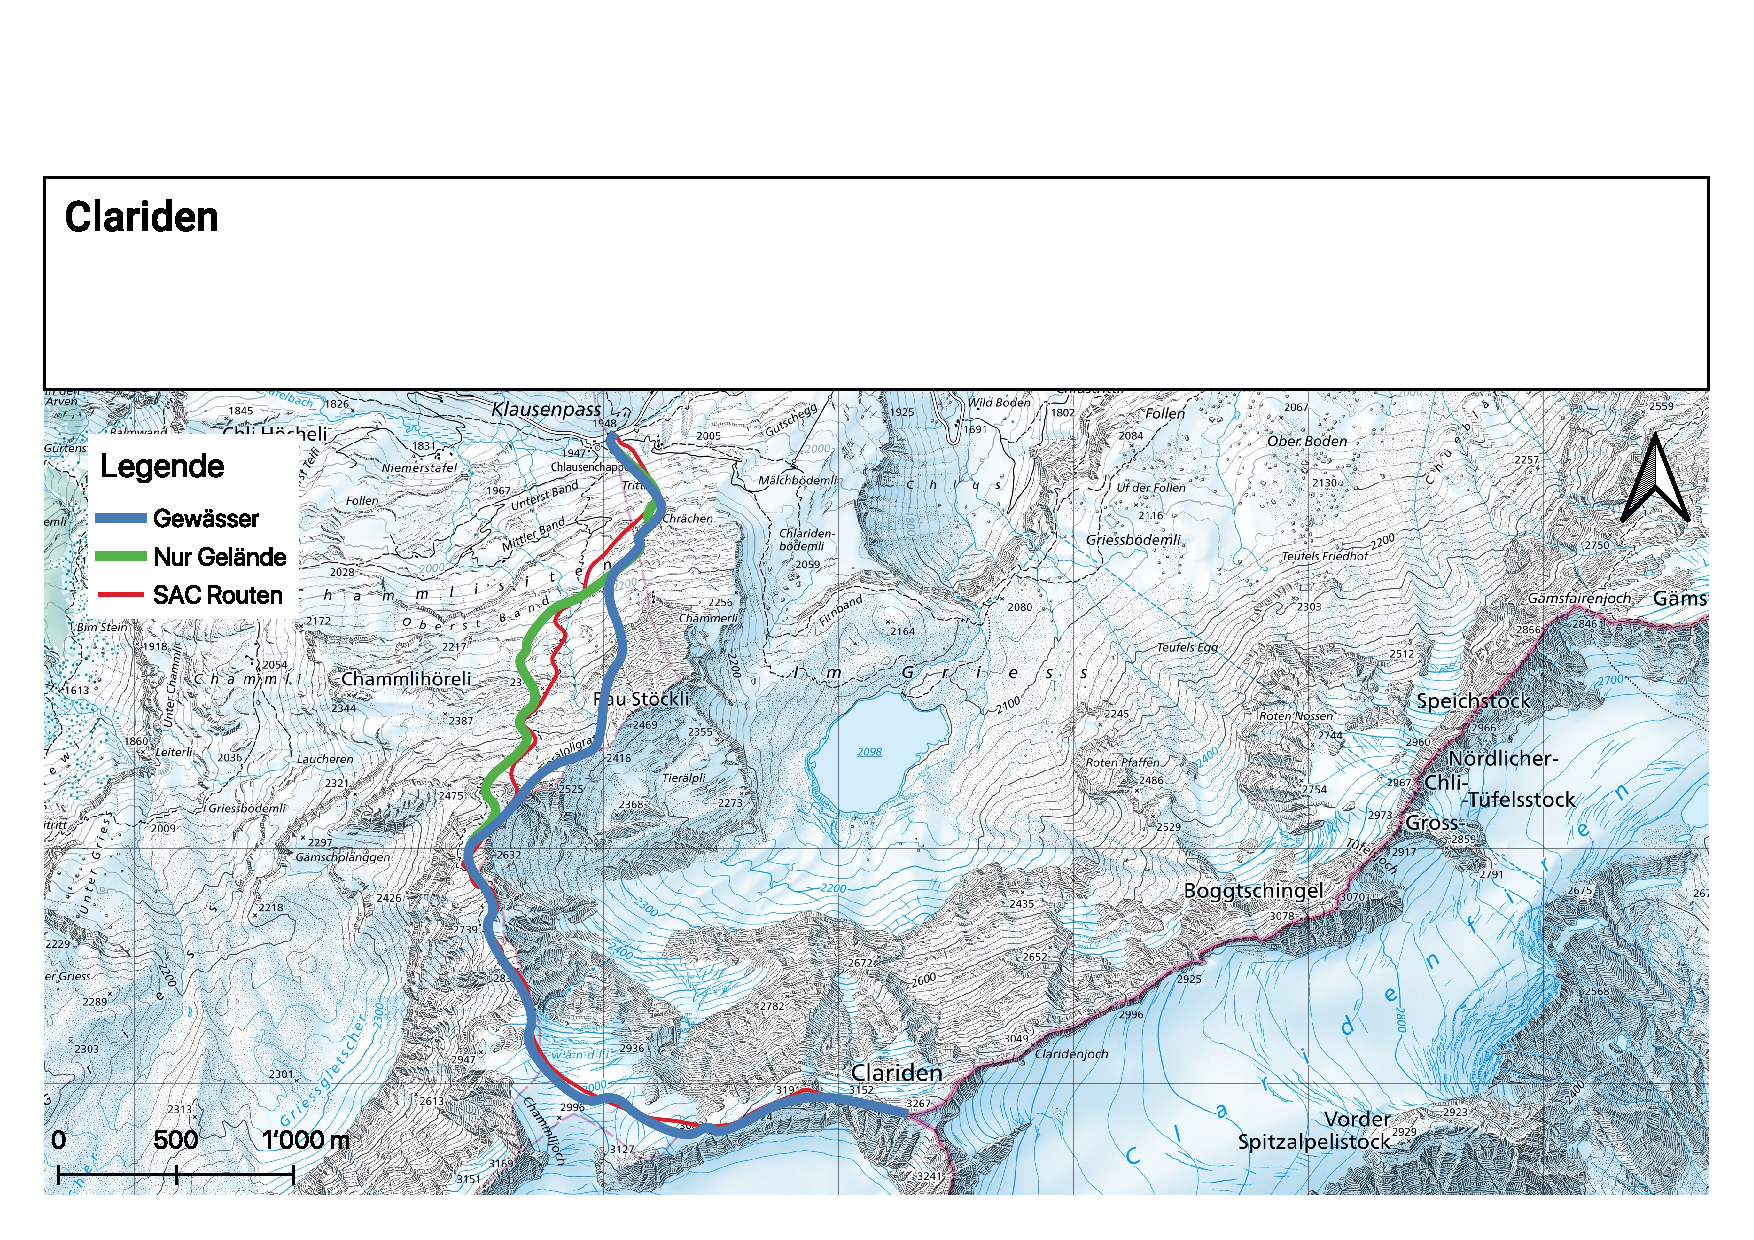
\includepdf[landscape=true]{./../evaluation/PDFs/Clariden.pdf}
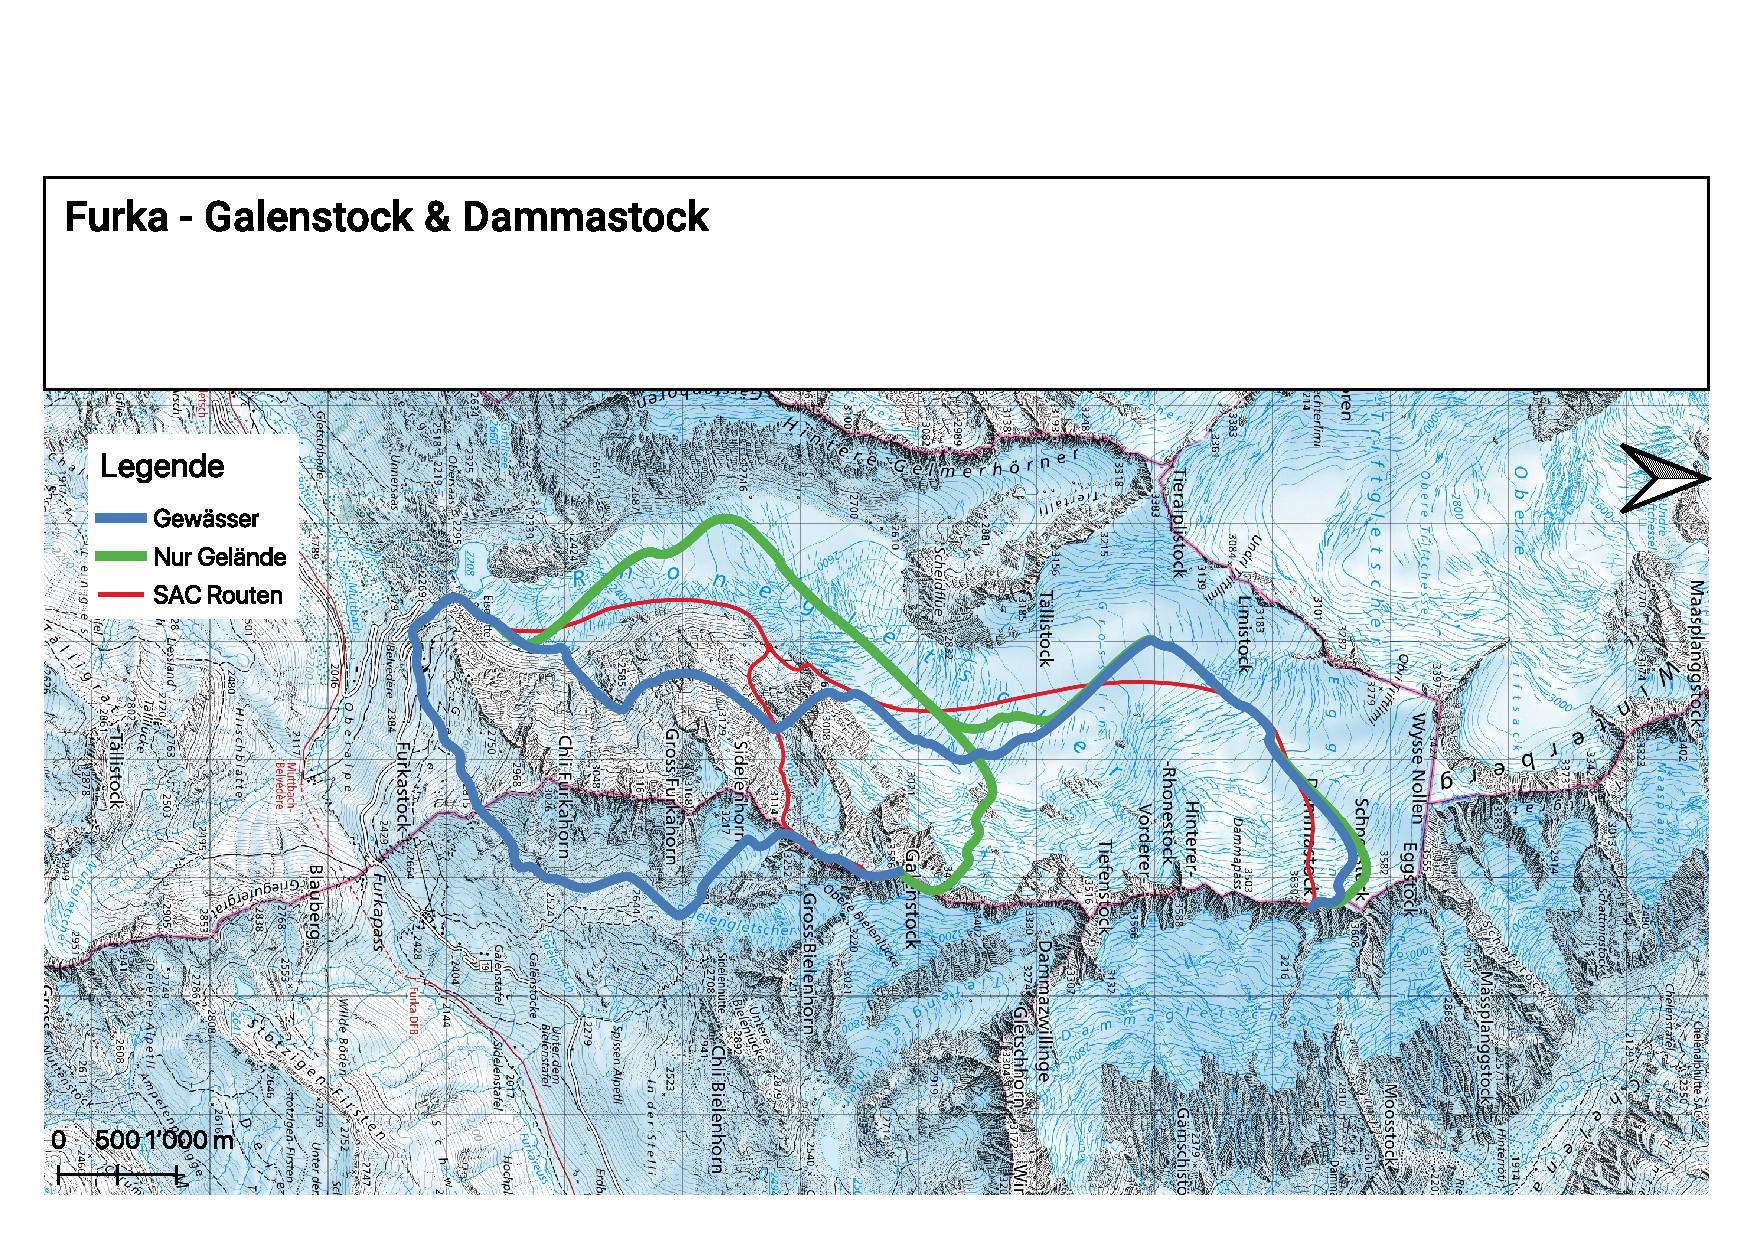
\includepdf[landscape=true]{./../evaluation/PDFs/Furka - Galenstock & Dammastock.pdf}
\includepdf[landscape=true]{./../evaluation/PDFs/Länta - Rheinwaldhorn_Adula.pdf}
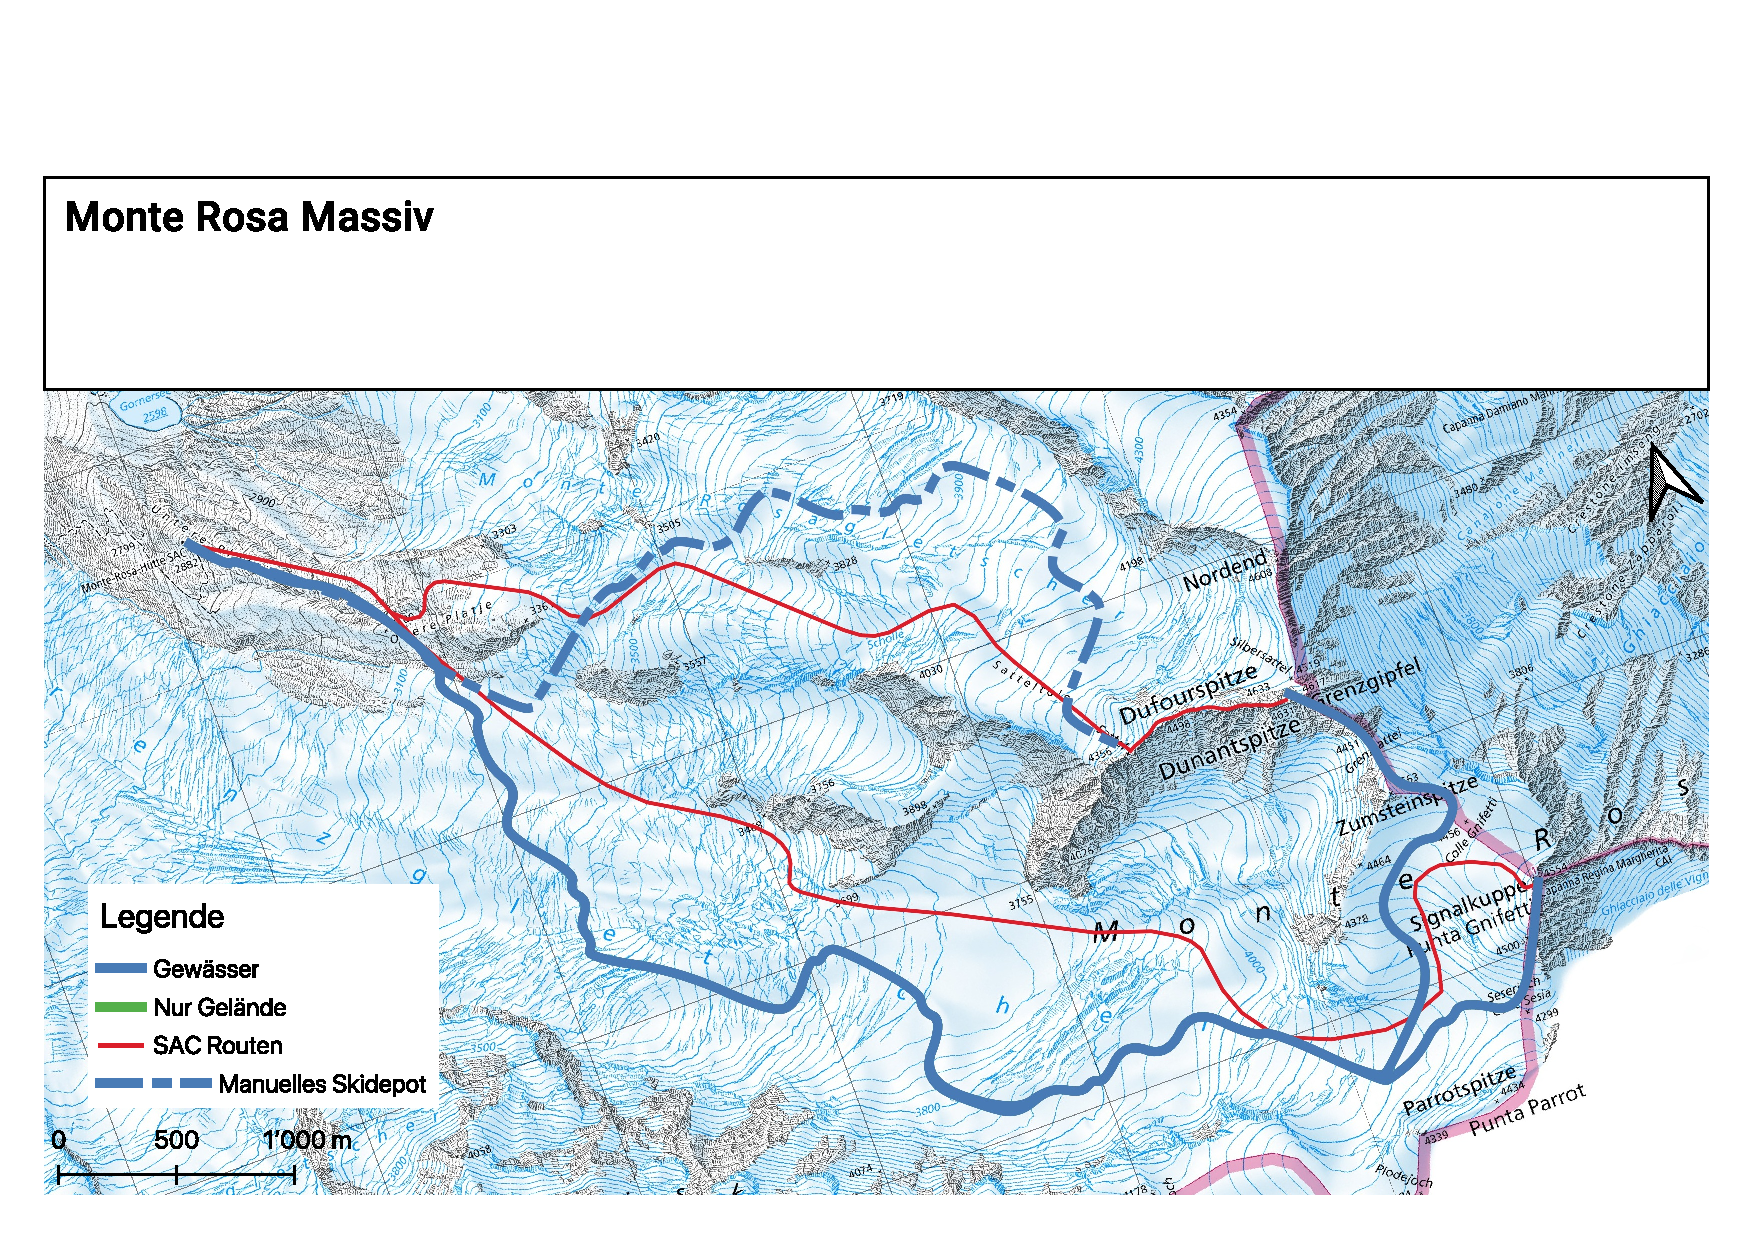
\includepdf[landscape=true]{./../evaluation/PDFs/Monte Rosa Massiv.pdf}
\includepdf[landscape=true]{./../evaluation/PDFs/Piz Palü.pdf}
\includepdf[landscape=true]{./../evaluation/PDFs/Strahlhorn.pdf}
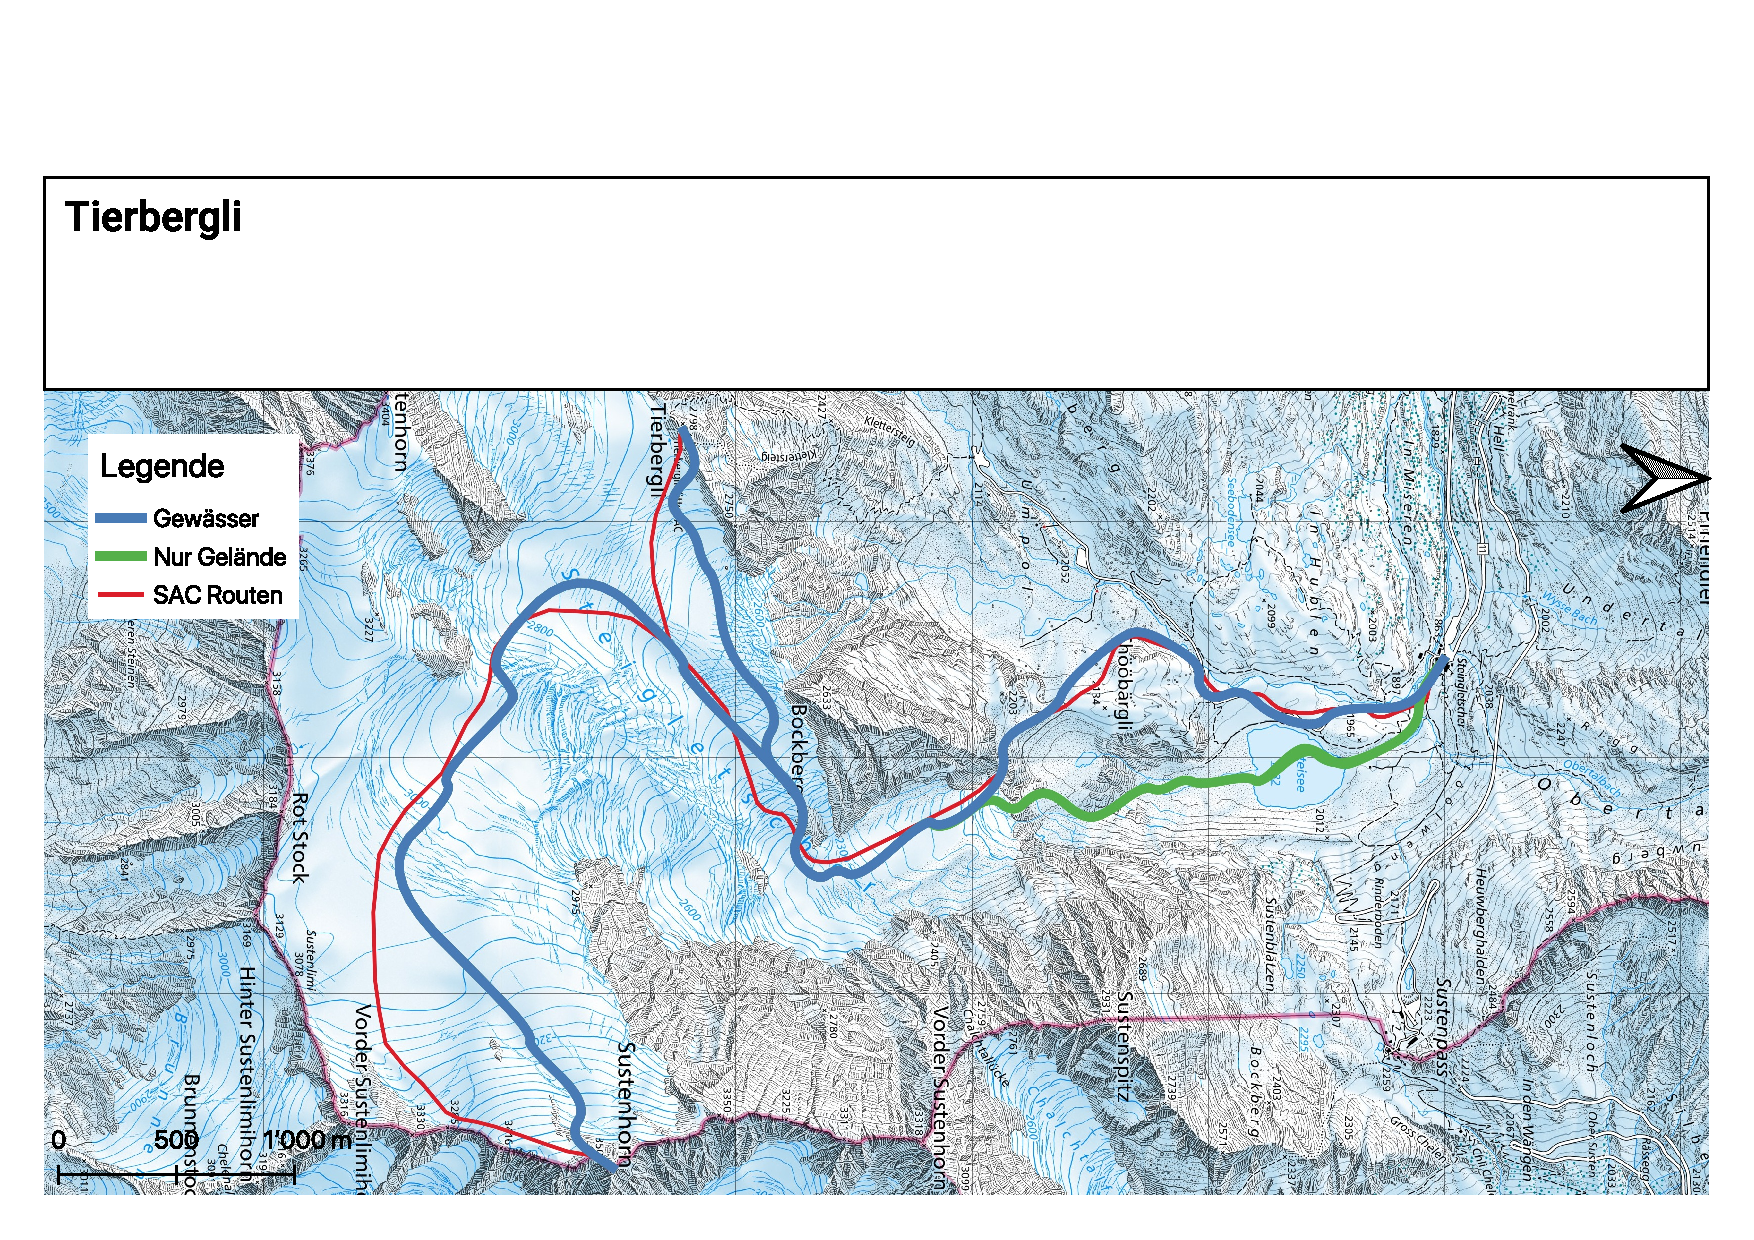
\includepdf[landscape=true]{./../evaluation/PDFs/Tierbergli.pdf}

\section{Lawinensimulation {RAMMS::Avalanche}}

\begin{figure}[H]
  \centering
  % \includegraphics[width=0.9\linewidth]{chelenalp_2d.gif}
  \caption{Python Code zur Produktion von Risikokarten aus Neigungskarte}\label{fig:chelenalp2d}
\end{figure}

\section{It's not a bug, it's a feature}